\newpage
\section{Supplementary materials} \label{supplementary}

\renewcommand{\thefigure}{S\arabic{figure}}
\setcounter{figure}{0}

\renewcommand{\thetable}{S\arabic{table}}
\setcounter{table}{0}



\begin{figure}[H]
    \centering
    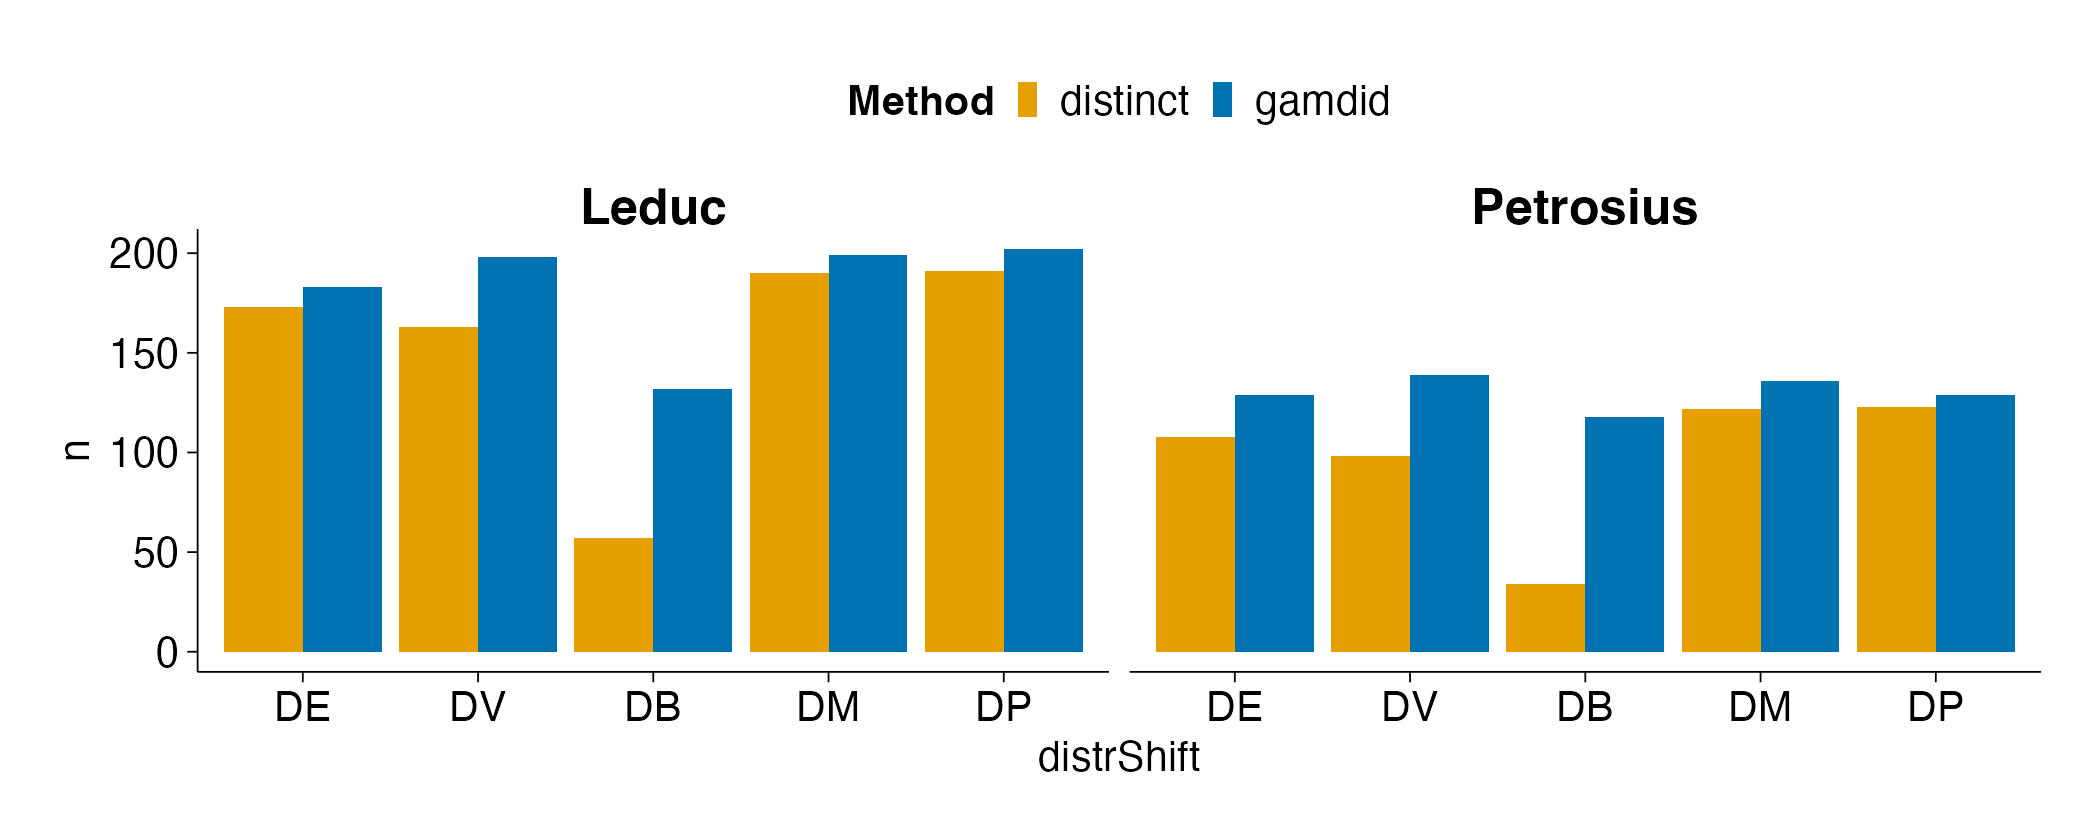
\includegraphics[width=0.85\linewidth]{figs/figS1.jpg}
    \captionsetup{labelfont={bf,small,color=red}}
    \caption{\textbf{\textcolor{red}{Absolute true positive counts for gamdid and distinct at 5\% FDR}} Bar charts displaying the number of true positives recovered at the nominal 5\% FDR threshold for gamdid and distinct across the five simulation scenarios in the Leduc dataset (left) and the Petrosius dataset (right). gamdid recovers a comparable or greater number of true positives in all scenarios, with the largest absolute gains in the DV and DB scenarios (shape-only differences). The false positive counts (Figure \ref{fig:FP}) are similarly low for both methods.}
    \label{fig:TP}
\end{figure}

\begin{figure}[H]
    \centering
    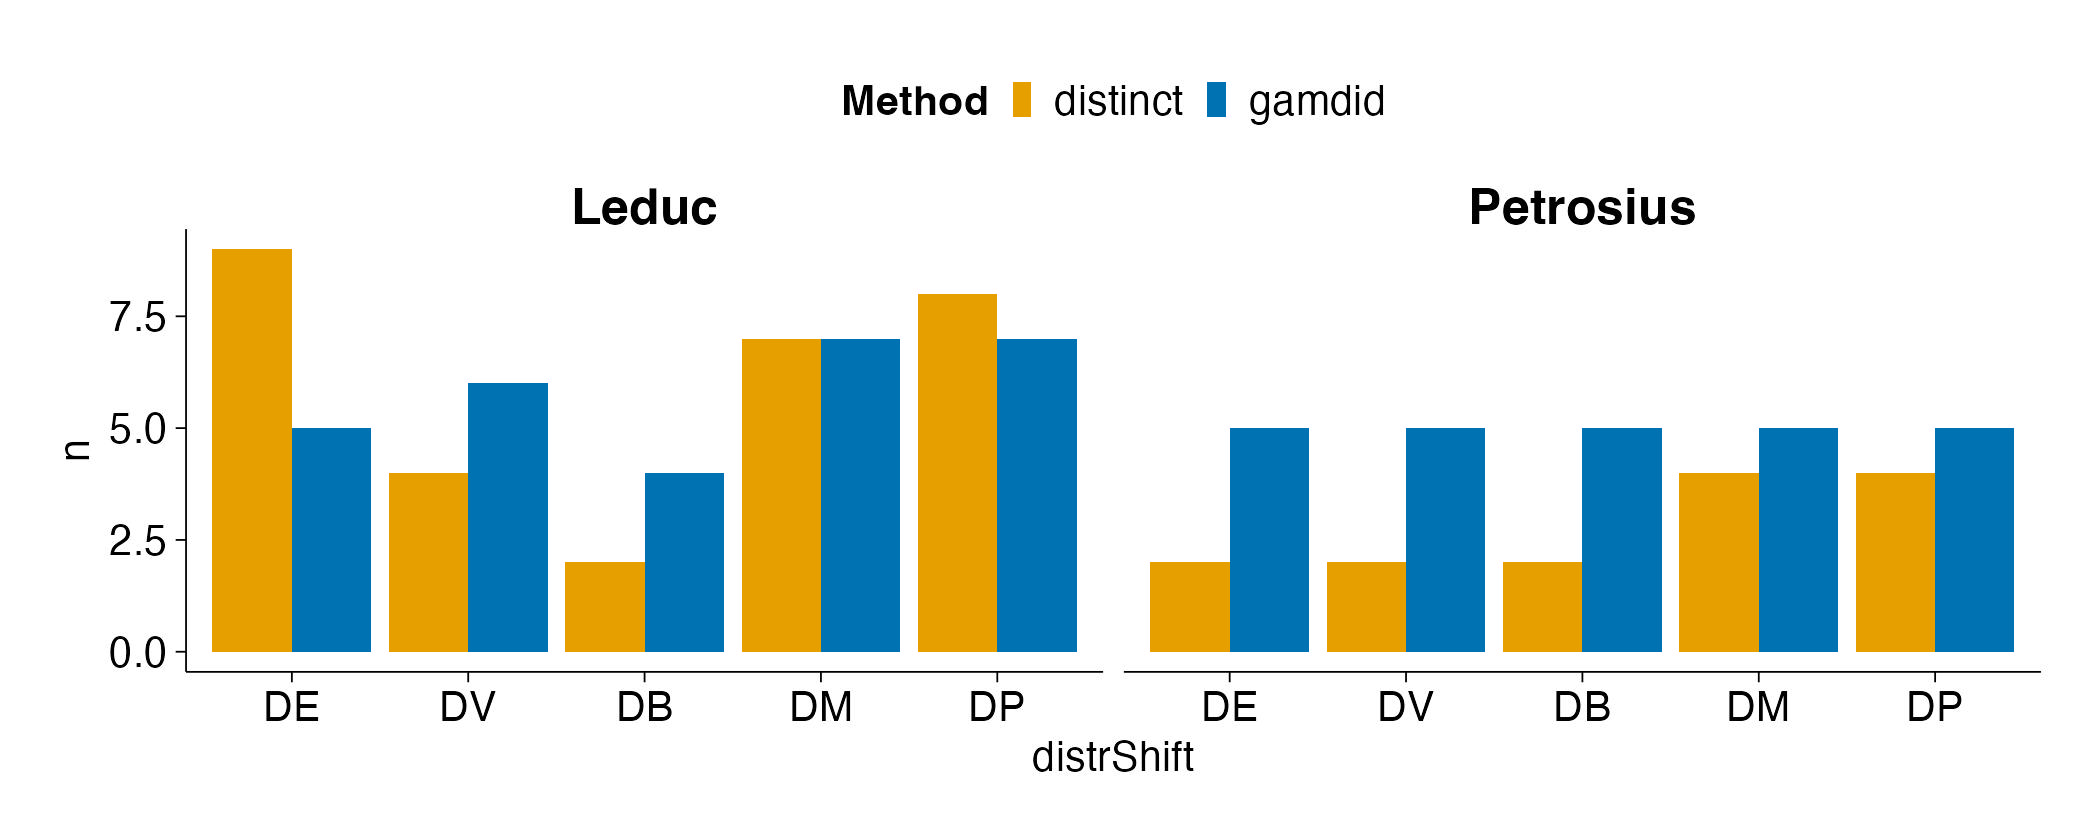
\includegraphics[width=0.85\linewidth]{figs/figS2.jpg}
    \captionsetup{labelfont={bf,small,color=red}}
    \caption{\textbf{\textcolor{red}{Absolute false positive counts for gamdid and distinct at 5\% FDR}} Bar charts displaying the number of false positives at the nominal 5\% FDR threshold for gamdid and distinct across the five simulation scenarios in the Leduc dataset (left) and the Petrosius dataset (right). Both methods maintain similarly low false positive counts across all scenarios in both datasets, confirming that the gains in true positive recovery demonstrated for gamdid in Figure \ref{fig:TP} are not accompanied by inflation of false discoveries.}
    \label{fig:FP}
\end{figure}

\begin{figure}[H]
    \centering
    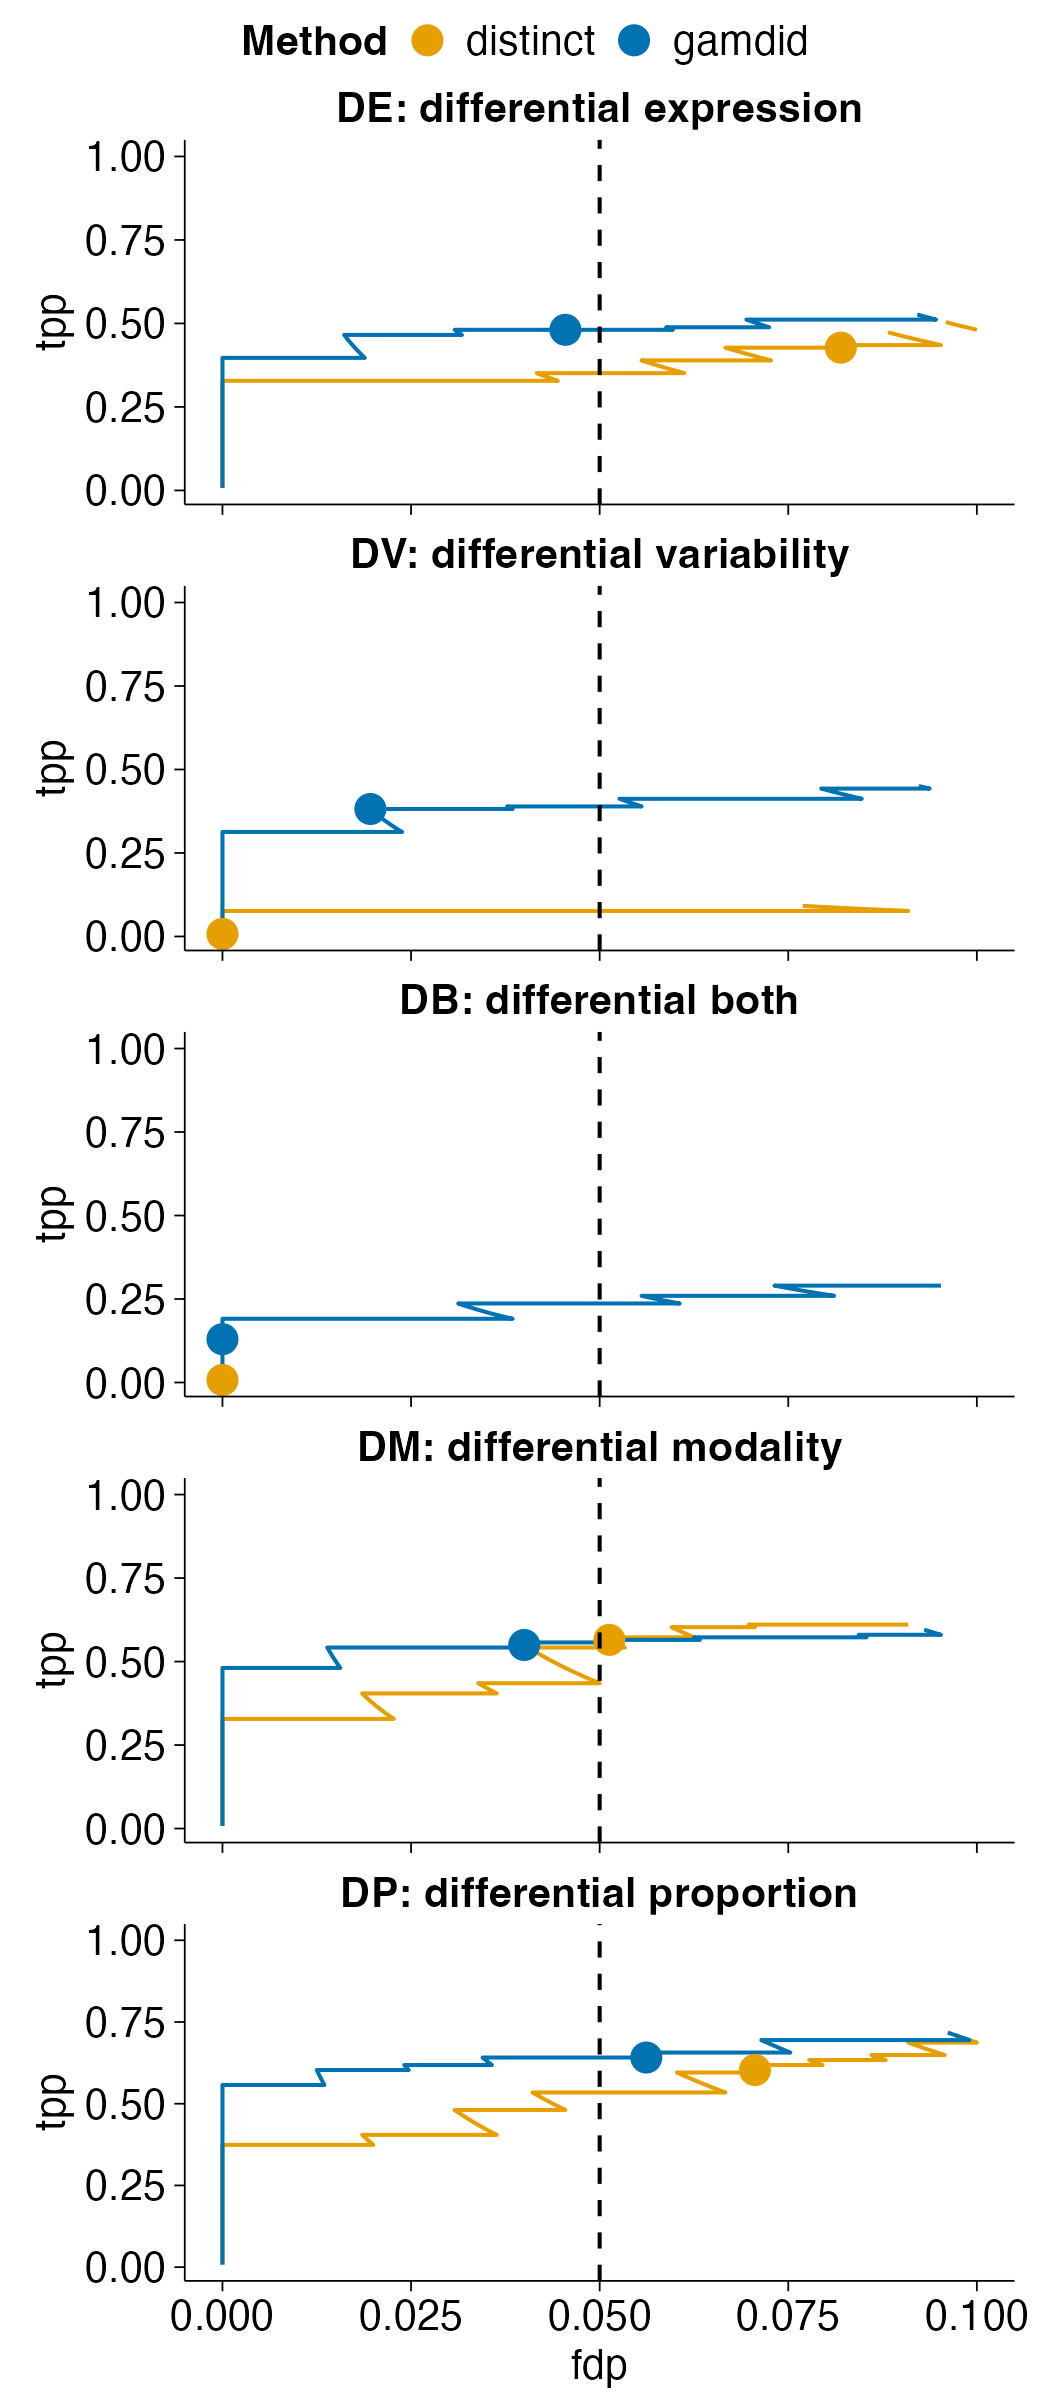
\includegraphics[width=0.425\linewidth]{figs/figS3.jpg}
    \caption{\textbf{Performance of gamdid on a subsampled Leduc dataset} FDP-TPP curves comparing gamdid and distinct across the five simulation scenarios, based on the protein-level mock data of a subsampled version of the Leduc dataset, in which cells were subsampled such that the average number of non-missing observations per group matched that of the Petrosius dataset. The dots mark the 5\% FDR threshold and the dashed vertical line marks FDP = 0.05. This analysis directly tests whether the more pronounced improvements of gamdid over distinct observed in the Petrosius dataset (see the right column of Figure \ref{fig:leducsims_gamdid}) are attributable to the smaller sample size. The results support this hypothesis: under reduced sample size, the performance gap between gamdid and distinct increases. distinct likely suffers from reduced null distribution resolution when fewer observations are available. DB (differential both) denotes a difference in both modality and component means.}
    \label{fig:leducsims_gamdid_subsample}
\end{figure}

\begin{figure}[H]
    \centering
    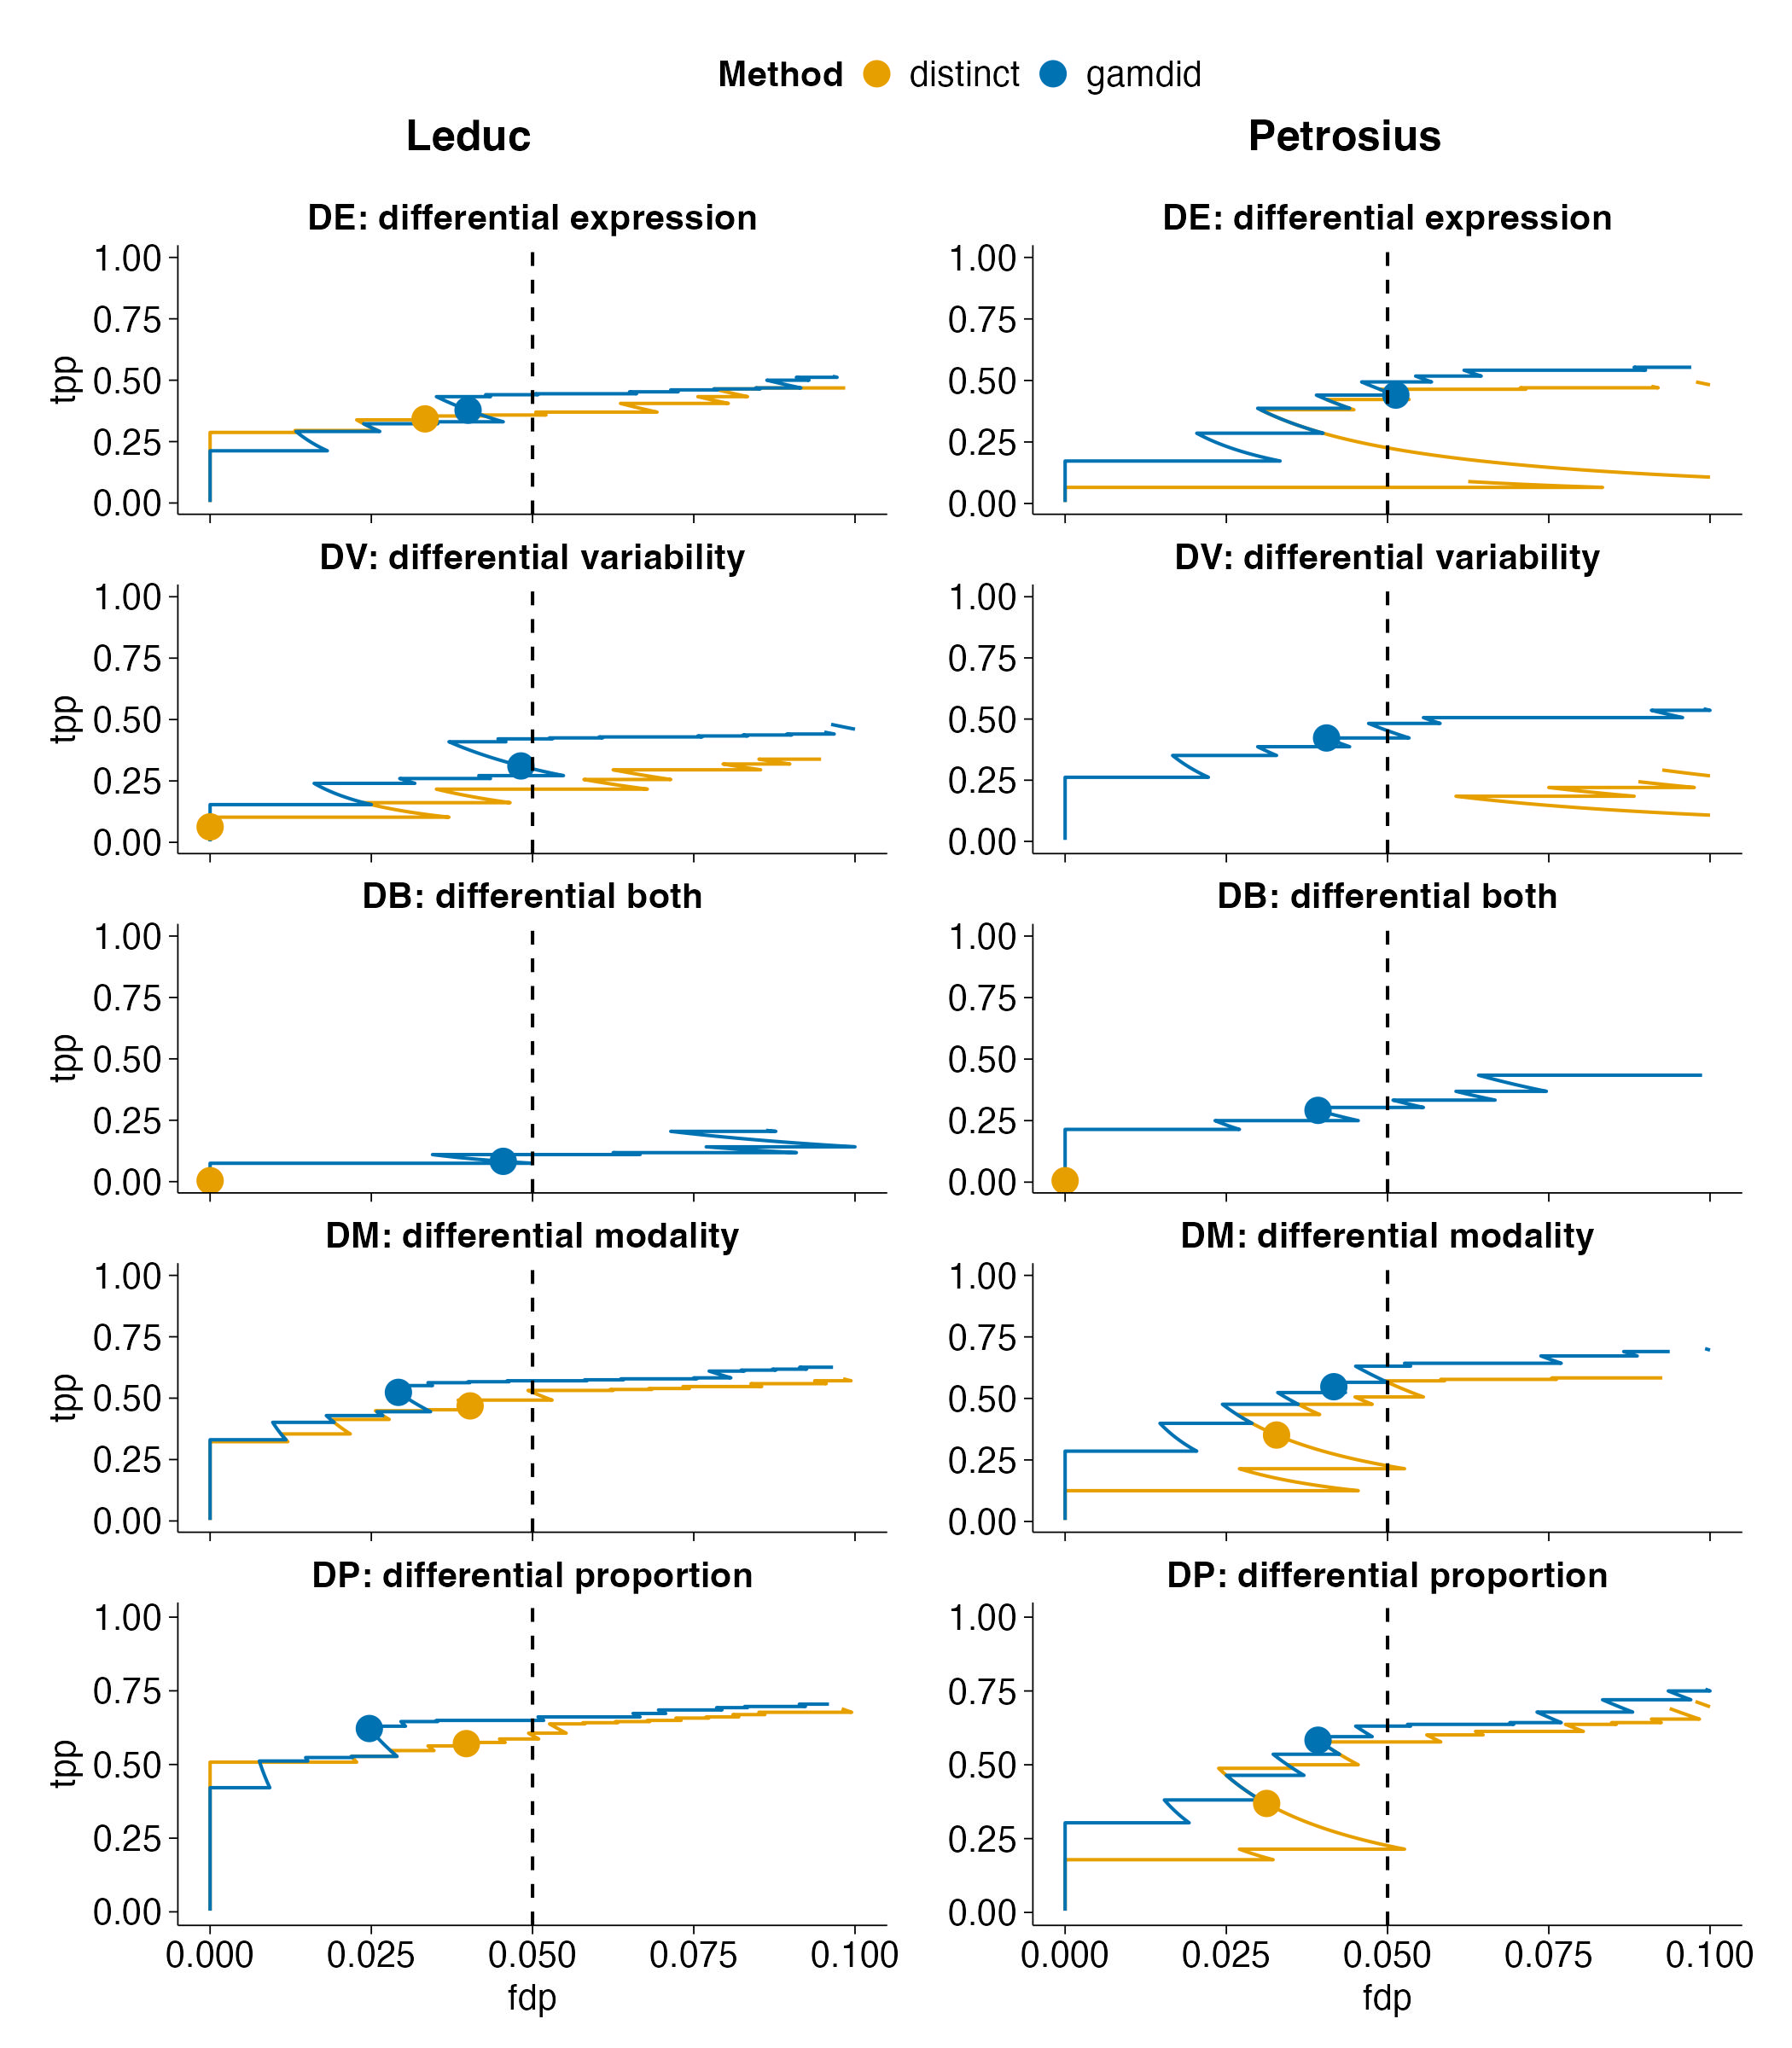
\includegraphics[width=0.85\linewidth]{figs/figS4.jpg}
    \captionsetup{labelfont={bf,small,color=red}}
    \caption{\textbf{\textcolor{red}{Performance of gamdid under reduced signal magnitude}} FDP-TPP curves comparing gamdid and distinct across the five simulation scenarios, based on the protein-level mock data of the Leduc dataset (left; 755 monocytes) and the Petrosius dataset (right; 269 m2i cells), under simulation scenarios with 25\% reduced signal magnitudes (DE: a shift of 30\% instead of 40\% of the feature's standard deviation was used; DV: random Gaussian noise with a standard deviation of 90\% of the feature's standard deviation was added instead of 120\%; DM and DB: a shift of 70\% of the feature's standard deviation was used instead of 90\%, and for DP 75\% instead of 100\%). The dots mark the 5\% FDR threshold and the dashed vertical line marks FDP = 0.05. This analysis assesses whether gamdid's performance advantages are robust to weaker signals that may be encountered in practice. The results are consistent with the original simulations (Figure \ref{fig:leducsims_gamdid}): gamdid controls the FDR at or below the nominal level and retains its advantages for shape-based distributional changes (DV, DB), while remaining competitive with distinct for scenarios where location shifts are involved. The relative improvements over distinct are more pronounced in the Petrosius dataset, consistent with gamdid's advantage under smaller sample sizes. As expected, the reduced signal does lower the overall power of both methods. DB (differential both) denotes a difference in both modality and component means.}
    \label{fig:leducsims_lower_gamdid}
\end{figure}


\begin{figure}[H]
    \centering
    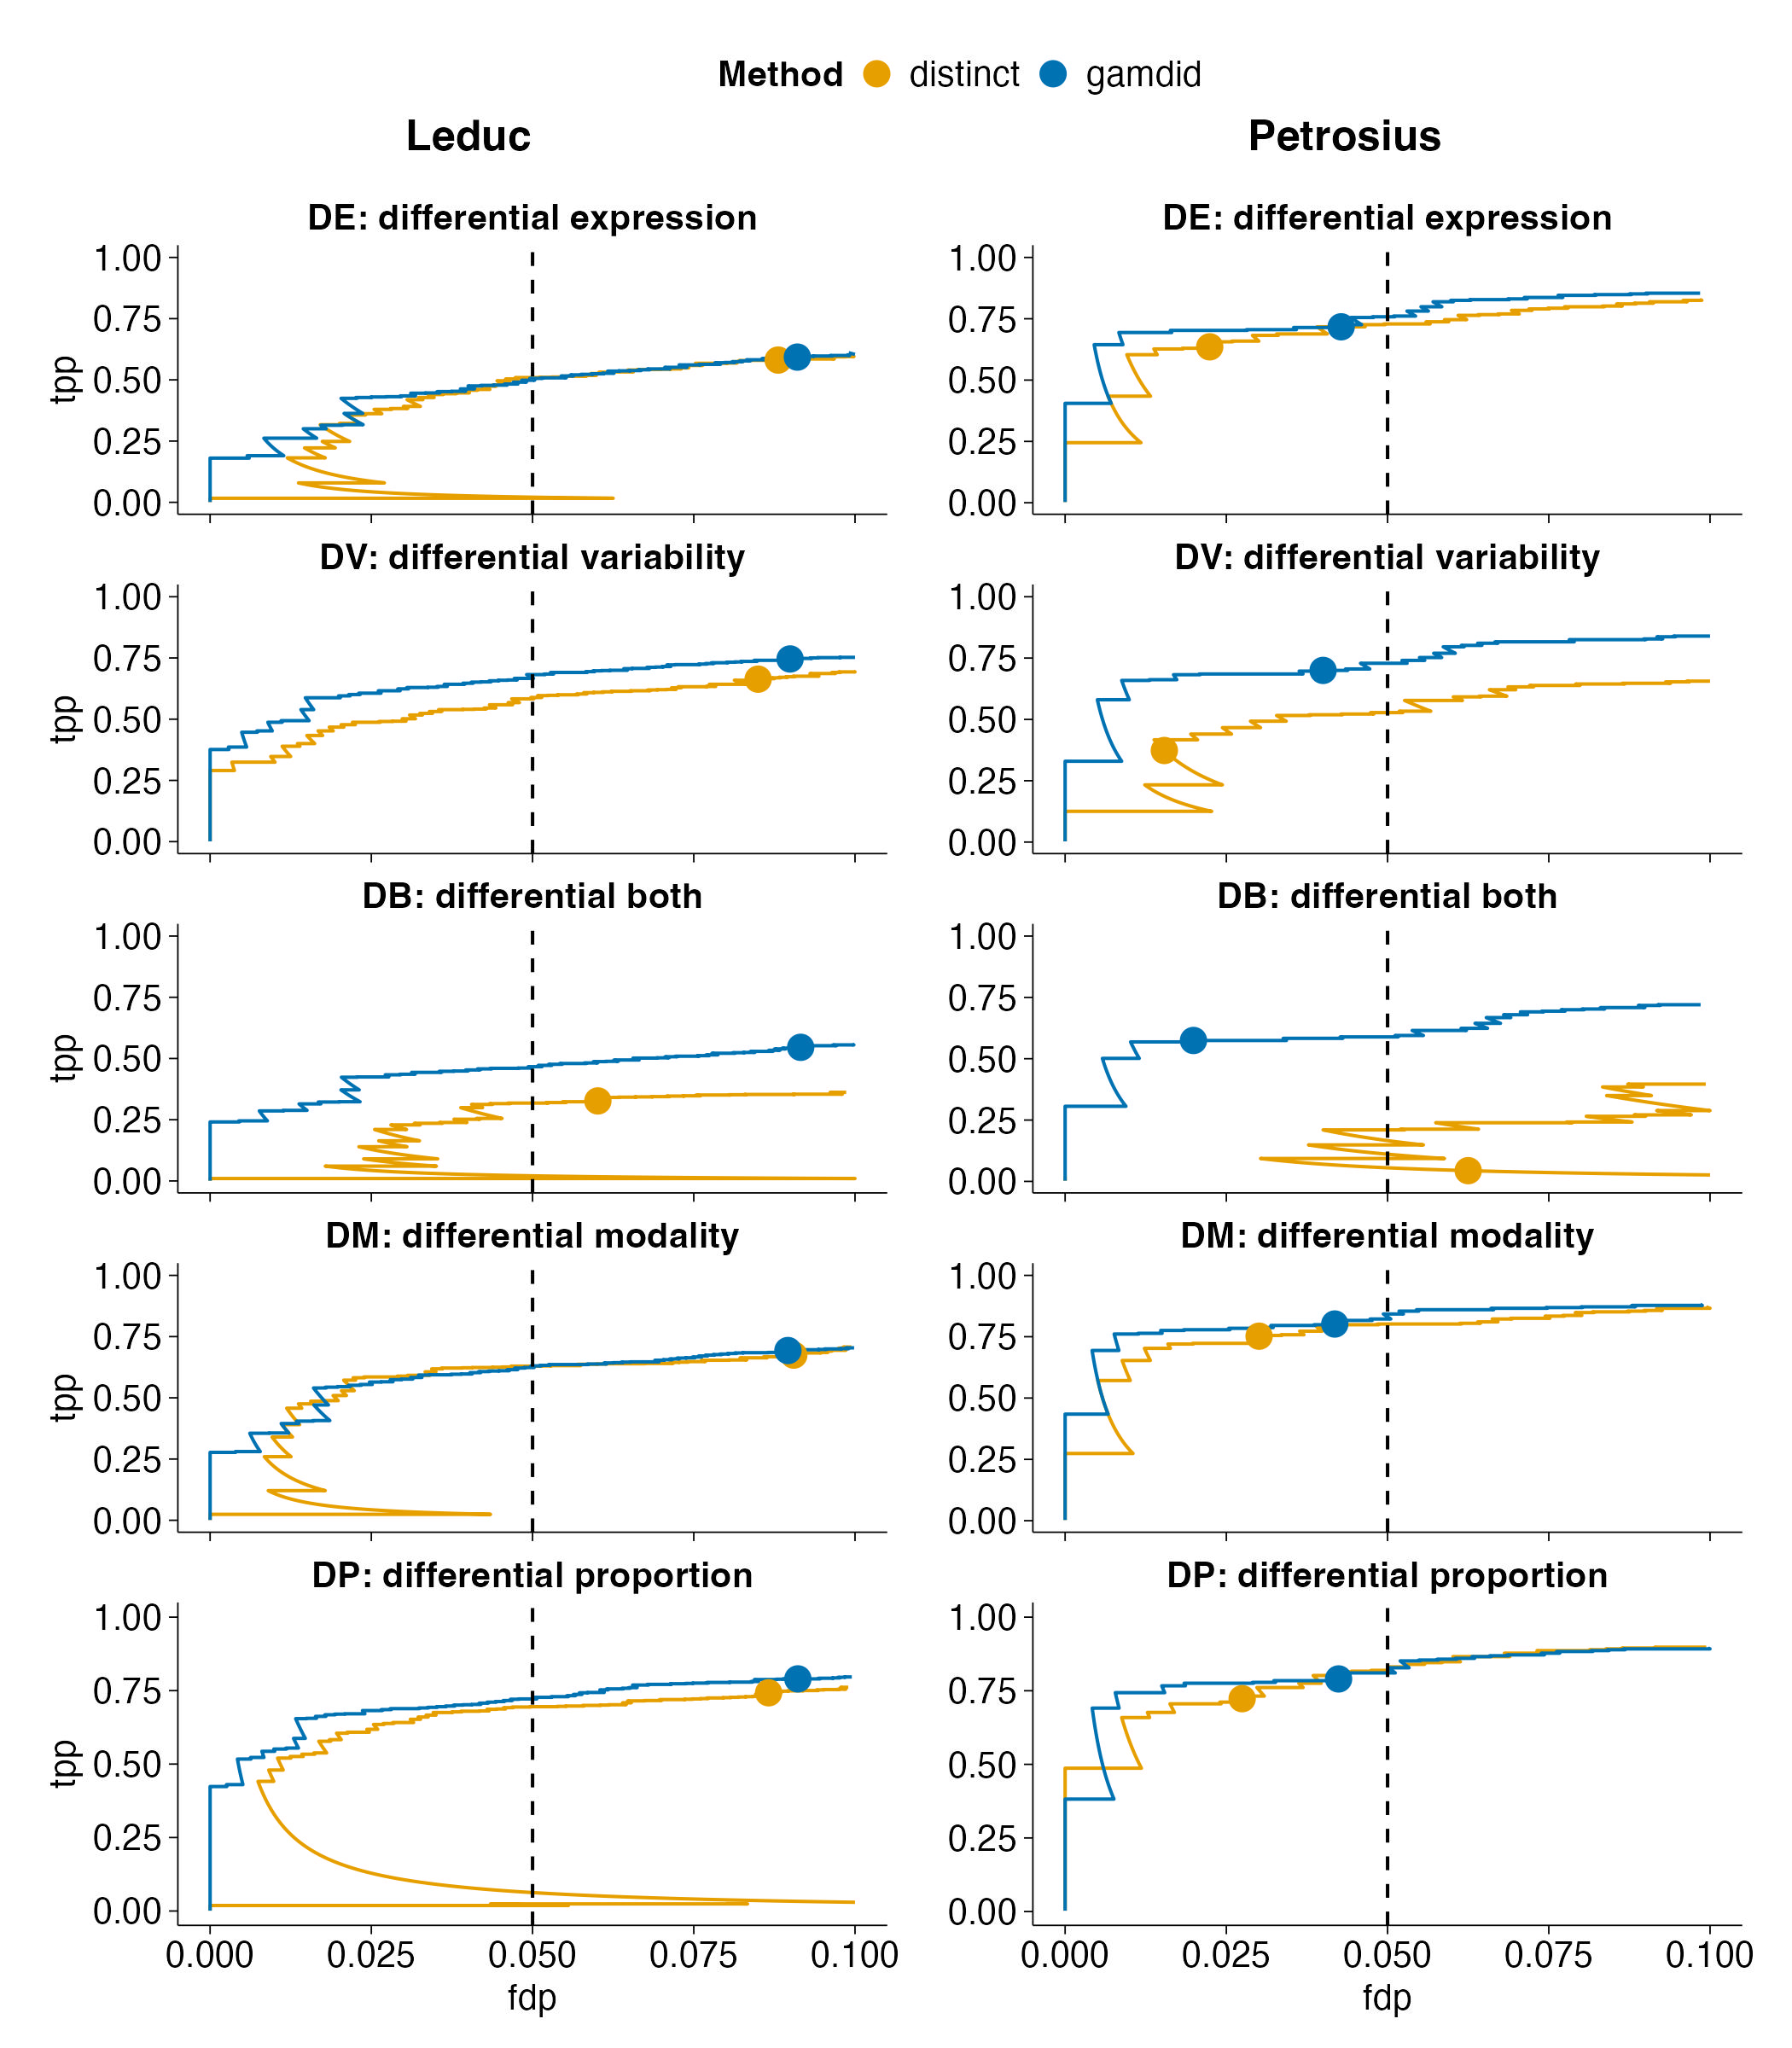
\includegraphics[width=0.85\linewidth]{figs/figS5.jpg}
    \captionsetup{labelfont={bf,small,color=red}}
    \caption{\textbf{\textcolor{red}{Performance of gamdid on peptide-level data}} FDP-TPP curves comparing gamdid and distinct across the five simulation scenarios, based on the peptide-level mock data of the Leduc dataset (left; 755 monocytes) and the Petrosius dataset (right; 269 m2i cells), rather than the protein-level summarized data used in the main analyses. The dots mark the 5\% FDR threshold and the dashed vertical line marks FDP = 0.05. The results are largely consistent with the protein-level findings (Figure \ref{fig:leducsims_gamdid}), and gamdid retains its performance advantages. In the Leduc dataset, FDR control is less conservative at the peptide level than at the protein level for both methods. This reflects the well-known challenge in peptide-level data: multiple peptides mapping to the same protein are correlated. In the Petrosius dataset, gamdid controls the FDR at the peptide level. Despite this, gamdid provides a flexible and applicable framework across all processing levels of proteomics data. DB (differential both) denotes a difference in both modality and component means.}
    \label{fig:leducsims_pep}
\end{figure}


\begin{figure}[H]
    \centering
    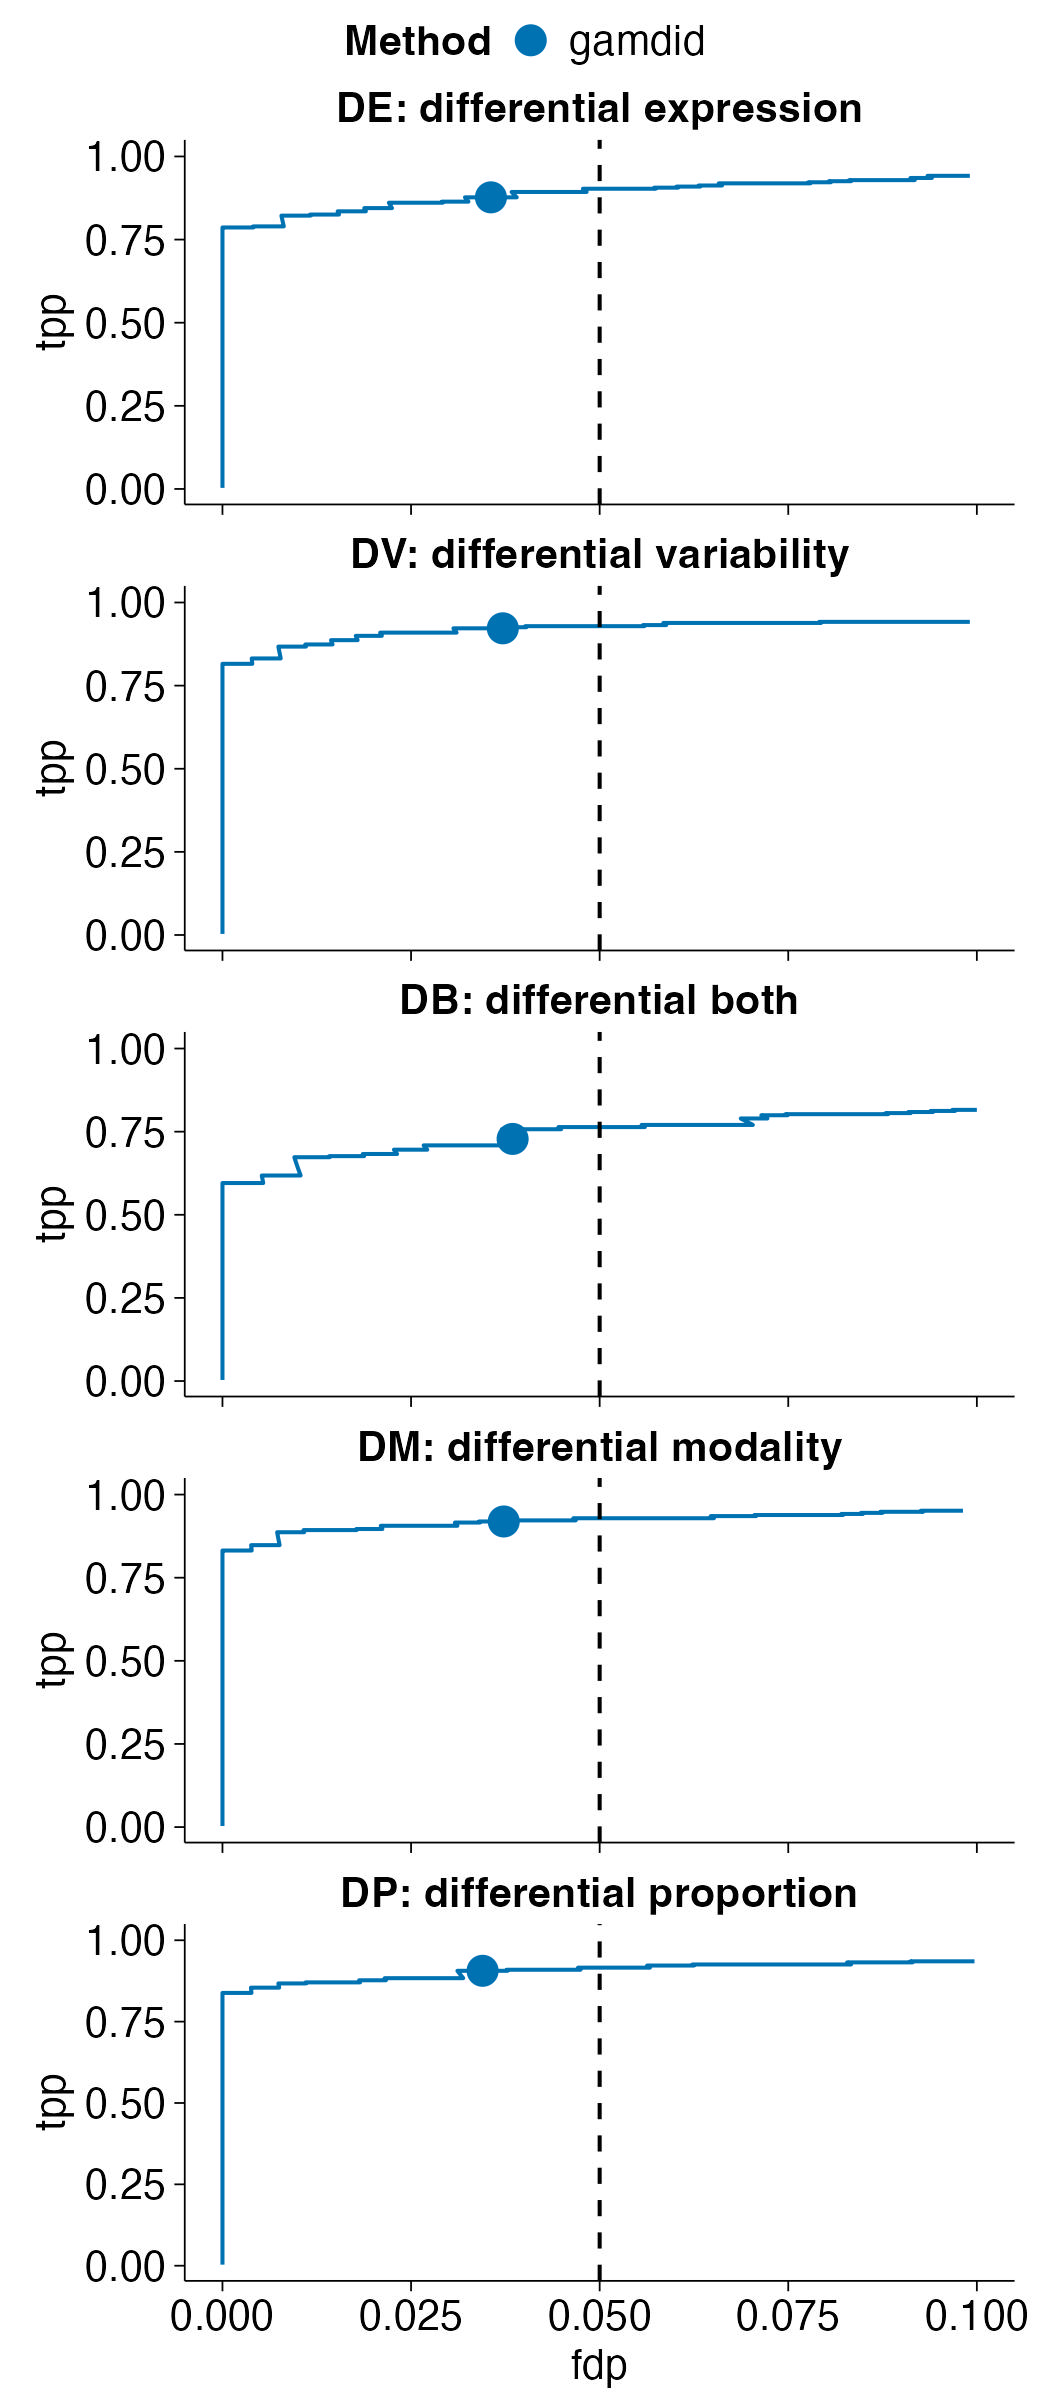
\includegraphics[width=0.425\linewidth]{figs/figS6.jpg}
    \caption{\textbf{Performance of the gamdid omnibus test in a three-group simulation} FDP-TPP curves for gamdid's omnibus test across the five simulation scenarios, based on the protein-level mock data of the Leduc dataset (755 monocytes). Cells were randomly assigned to three mock groups (A, B, C), with distributional signal introduced in group B under the same five simulation scenarios as in the two-group analyses. No competing DD method currently supports multi-group omnibus testing, so no benchmark comparison is possible here; these curves demonstrate gamdid's standalone performance in this setting. The dots mark the 5\% FDR threshold and the dashed vertical line marks FDP = 0.05. Notably, the three-group omnibus test achieves higher power than the corresponding two-group comparisons in the left column of Figure \ref{fig:leducsims_gamdid}. DB (differential both) denotes a difference in both modality and component means.}
    \label{fig:leduc_threegroup}
\end{figure}


\begin{table}[htbp]
\centering
\begin{tabular}{ccc}
\hline
\texttt{msqrob2} & \texttt{gamdid} & \texttt{distinct} \\
\hline
0.030\rlap{$^{*}$} & 0.055 & 0.039\rlap{$^{*}$}\\
0.046\rlap{$^{*}$} & 0.081 & 0.160\\
0.048\rlap{$^{*}$} & 0.081 & 0.039\rlap{$^{*}$}\\
0.048\rlap{$^{*}$} & 0.084 & 0.141\\
0.049\rlap{$^{*}$} & 0.083 & 0.055\\
0.049\rlap{$^{*}$} & 0.086 & 0.128\\
\\
0.149 & 0.090 & 0.035\rlap{$^{*}$}\\
0.128 & 0.197 & 0.039\rlap{$^{*}$}\\
\hline
\end{tabular}
\caption{\textbf{FDR-corrected p-values for features detected by msqrob2 and/or distinct but not by gamdid in the spike-in case study} The eight features that are flagged as significant by msqrob2 and/or distinct but not by gamdid are listed with their FDR-corrected p-values from all three methods. We see that gamdid consistently returns borderline non-significant p-values for the six features detected by msqrob2. In contrast, distinct produces both relatively high and relatively low p-values for these features. This indicates that only gamdid largely preserves the msqrob2 ranking of DA features. Significant FDR-corrected p-values ($<$ 0.05) are marked with an asterisk (*).}
\label{tab:only_msqrob2}
\end{table}

\begin{table}[htbp]
\centering
\begin{tabular}{ccc}
\hline
\texttt{msqrob2} & \texttt{gamdid} & \texttt{distinct} \\
\hline
0.931 & 0.028\rlap{$^{*}$} & 0.499\\
0.401 & 0.034\rlap{$^{*}$} & 0.067\\
0.074 & 0.045\rlap{$^{*}$} & 0.073\\
\hline
\end{tabular}
\caption{\textbf{FDR-corrected p-values for the three features detected exclusively by gamdid in the spike-in case study} The three features uniquely identified as significant by gamdid, with FDR-corrected p-values from all three methods. Two of the three features receive very high msqrob2 p-values, confirming that these differences do not involve a detectable mean shift and would be entirely missed by any conventional DA approach. Significant FDR-corrected p-values ($<$ 0.05) are marked with an asterisk (*).}
\label{tab:only_gamdid}
\end{table}

\clearpage
\begin{figure}[H]
    \centering
    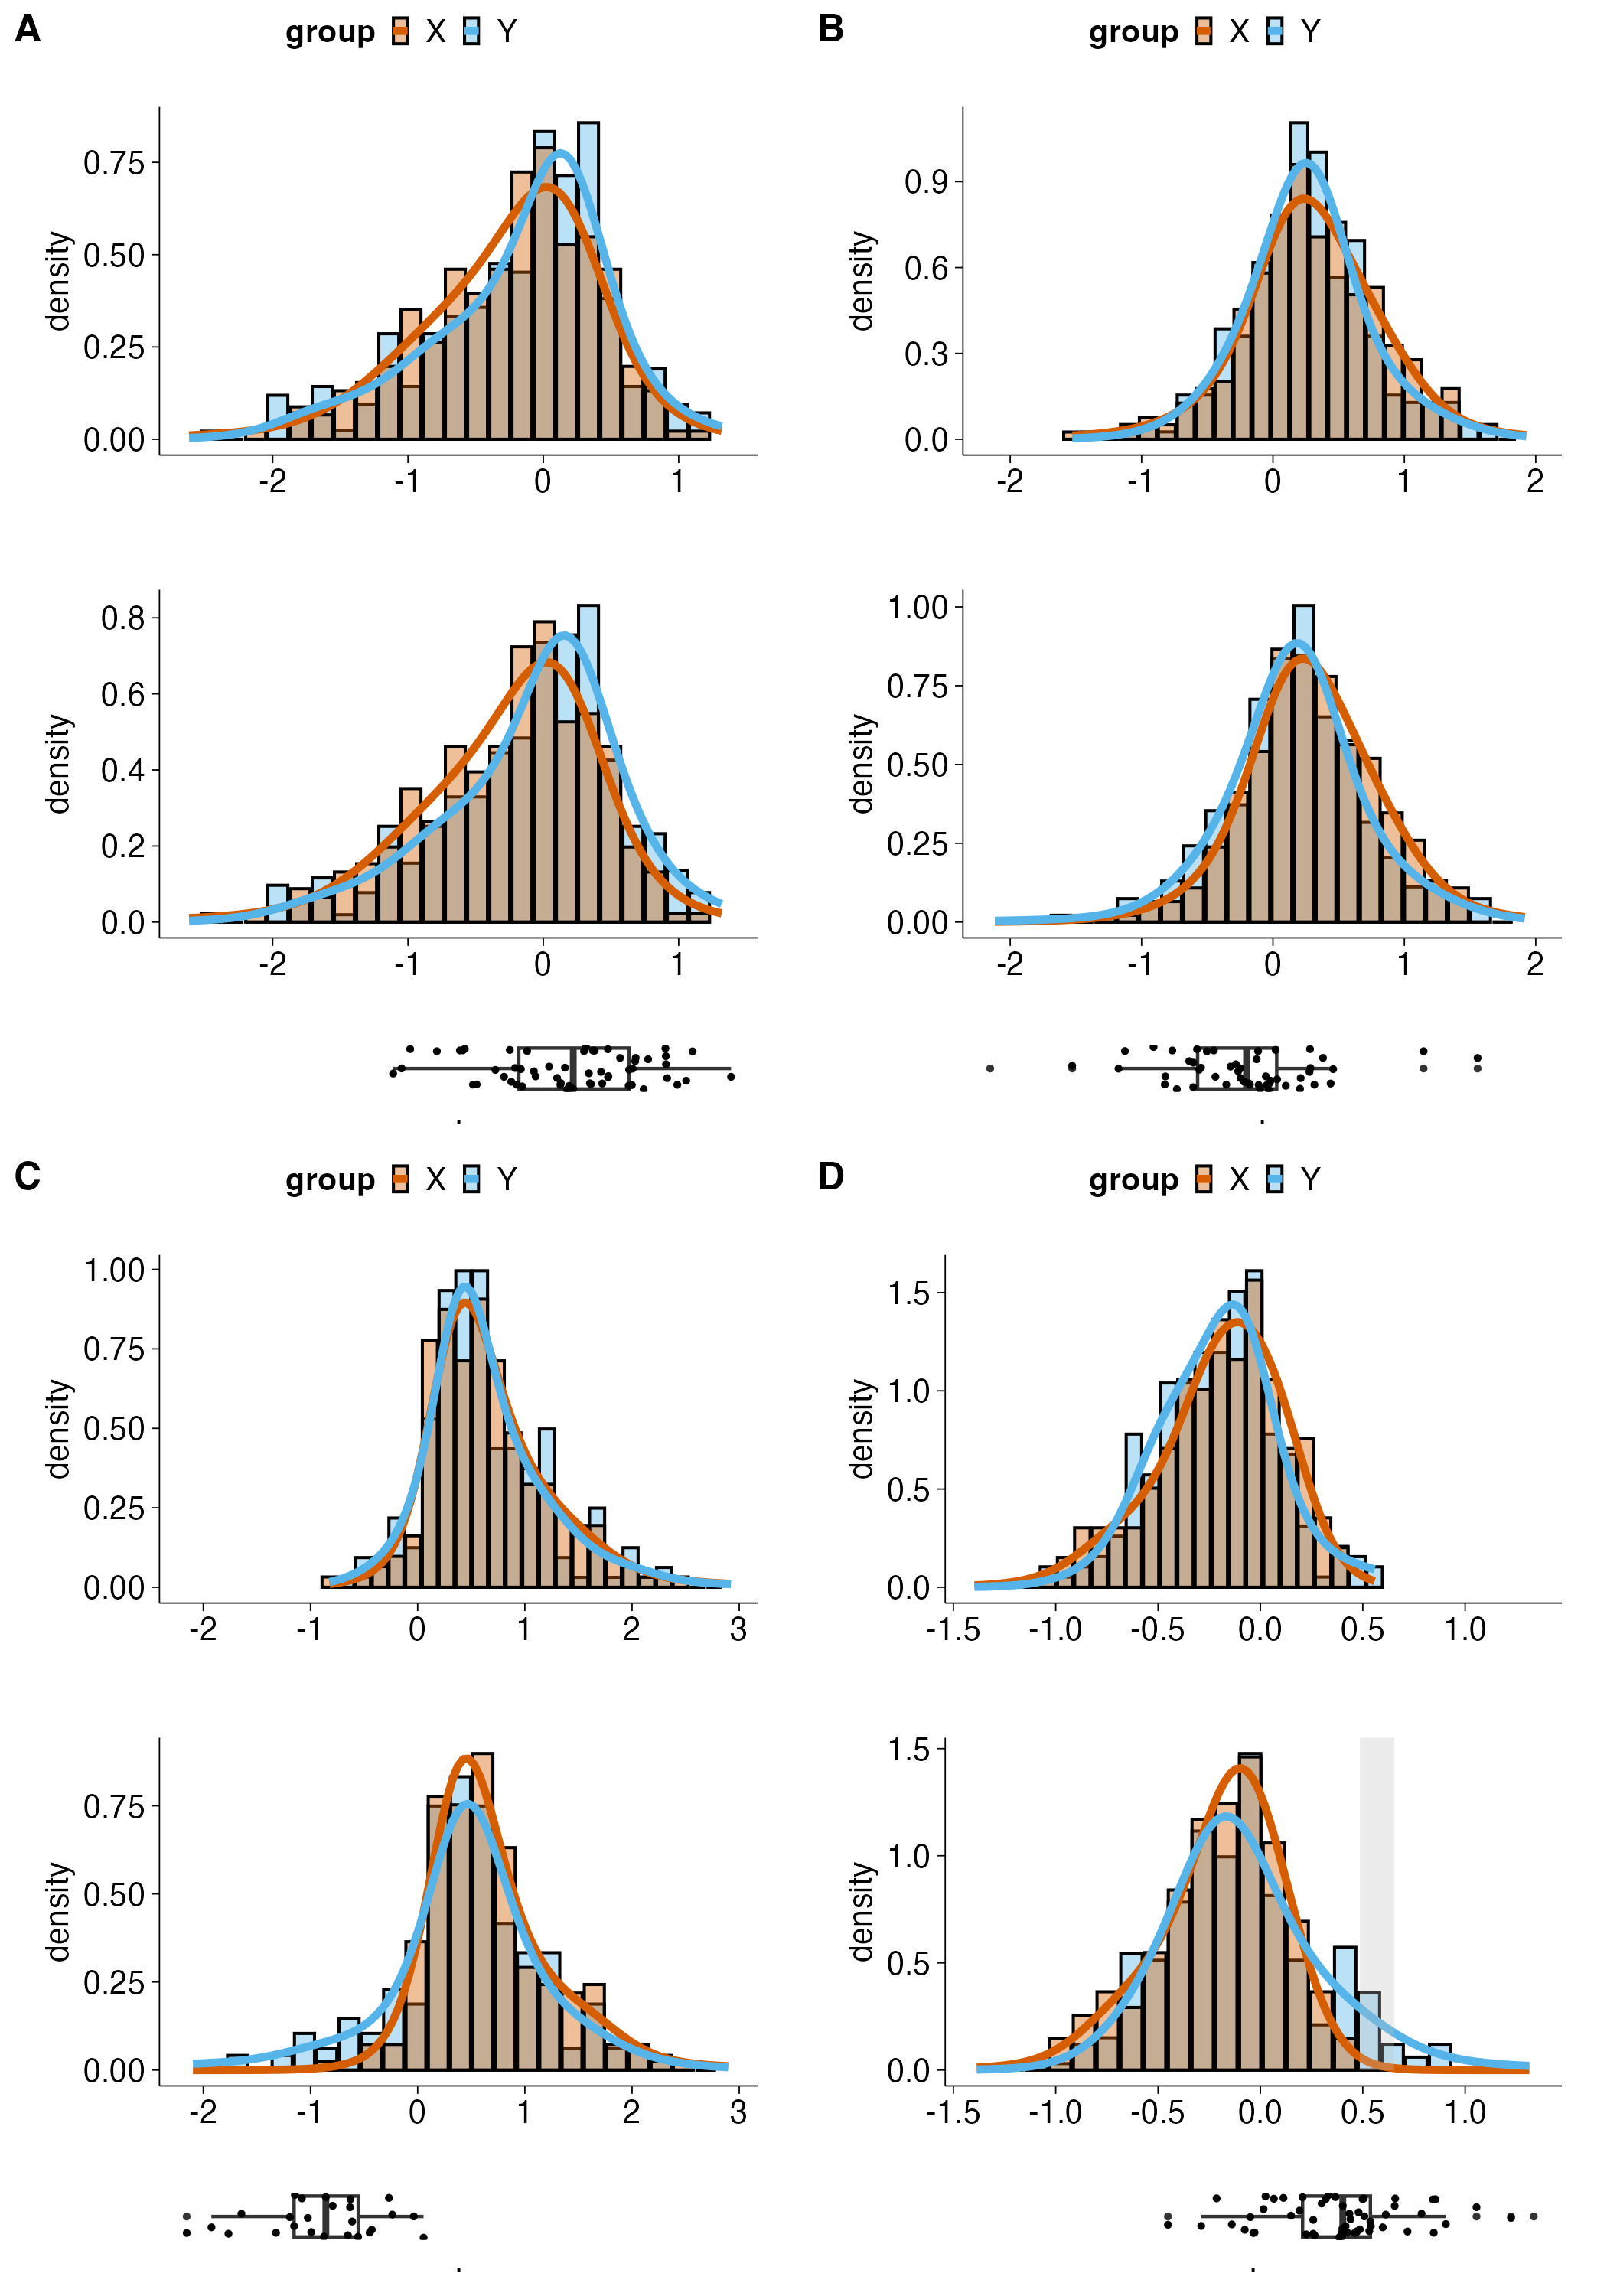
\includegraphics[width=0.85\linewidth,height=0.75\textheight,keepaspectratio]{figs/figS7.jpg}
    \captionsetup{labelfont={bf,small,color=red}}
    \caption{\textbf{\textcolor{red}{gamdid visualizations for features detected only by msqrob2 or only by distinct in the spike-in case study}} The output of gamdid's visFit function for two of the four features flagged as significant exclusively by msqrob2 (\textbf{A}, \textbf{B}) and the two features flagged as significant exclusively by distinct (\textbf{C}, \textbf{D}). Each panel shows the mock comparison (top), in which the groups show no distributional difference, the comparison after spiking 10\% of the 697 sub-cluster A melanoma cells (69 cells) into group Y (middle), and a boxplot indicating where the spike-in melanoma cells are located (bottom). \textbf{A--B}: After spike-in, a weak mean shift appears, but no differential region is found by gamdid (no gray shading). This illustrates a feature type where msqrob2's dedicated sensitivity for mean shifts gives it a slight edge over gamdid. \textbf{C}: After spike-in, the melanoma cells add a heavier left tail to the distribution of group Y, but no differential region is found by gamdid (no gray shading). Here, distinct's ECDF-based approach accumulates sufficient evidence to reach significance, while gamdid's local density approach does not identify a sufficiently concentrated differential region. \textbf{D}: After spike-in, the density of group Y shifts in the right tail, and gamdid's difference smoother identifies a differential region (gray shading), despite the FDR-corrected p-value being non-significant (gamdid FDR adjusted p-value = 0.090).}
    \label{fig:msqrob_distinct_only}
\end{figure}
\clearpage




\begin{figure}[H]
    \centering
    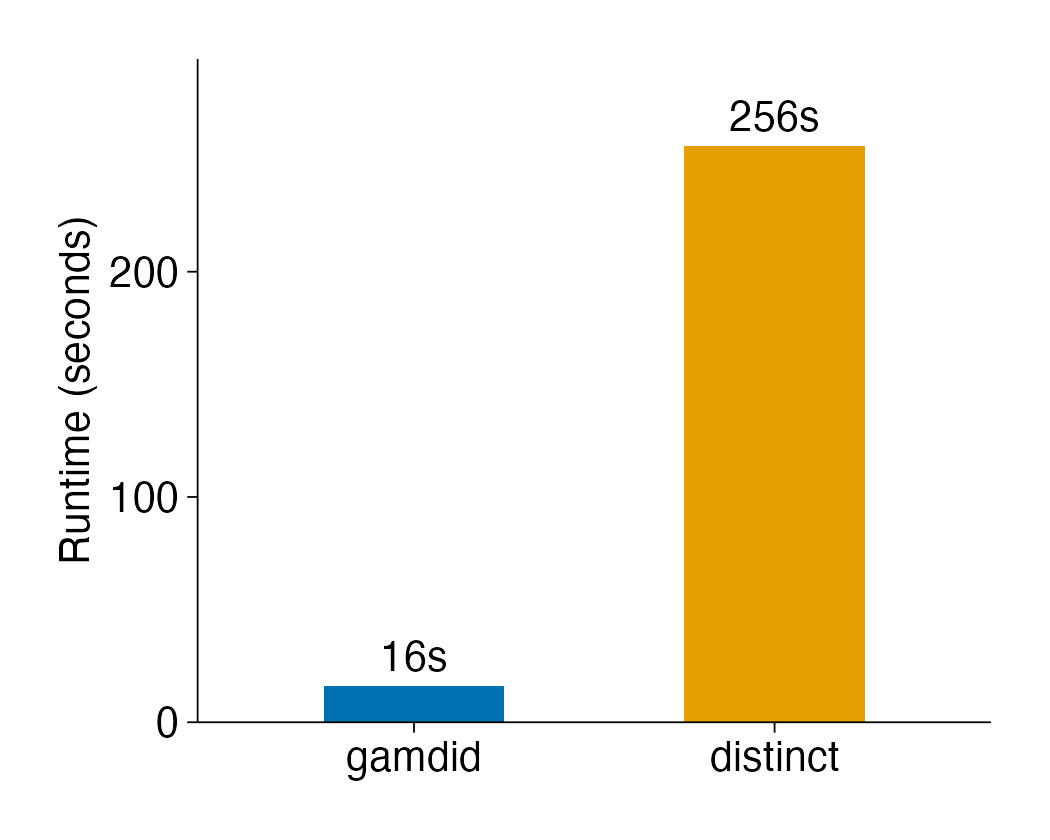
\includegraphics[width=0.425\linewidth]{figs/figS8.jpg}
    \caption{\textbf{Computational efficiency of gamdid and distinct}
    Mean runtime for gamdid and distinct on the spike-in case study dataset
    (1316 features, 824 cells), each run on a single core and averaged
    across ten independent runs. gamdid completed in 16 seconds on average,
    whereas distinct required 256 seconds, corresponding to a more than
    fifteen-fold speedup.}
  \label{fig:runtime}
\end{figure}

\subsection{\texorpdfstring{\textcolor{red}{Supplementary methods: full statistical derivation}}{Supplementary methods: full statistical derivation}} \label{suppl_methods}

\textcolor{red}{This section provides the details underlying the \texttt{gamdid} approach summarized in the Methods section.} We first detail the density estimation approach and the Poisson generalized additive model used. We subsequently describe the inference procedure and the p-value aggregation strategy. Next we elaborate on the post-hoc pairwise comparisons and stagewise testing procedure, followed by the approach for identifying regions of differential density.

\subsubsection{Model and inference}

The statistical methodology for comparing distributions is developed for a single feature (in this case proteins or peptides). The method is then simply repeated over multiple features and the corresponding p-values are corrected for multiple testing using the conventional Benjamini-Hochberg FDR procedure \cite{BH_procedure} or stagewise testing \cite{stagewise_testing}.
\\
\\
\textbf{Density estimation through Poisson regression} Following the approach of Lindsey \cite{lindsay_method}, we reformulate density estimation in terms of Poisson regression by discretizing the sample space. We partition the sample space $\mathscr{Y}$ into $K$ disjoint bins $\mathscr{Y}_k$ of equal width $bw$.

\begin{equation}
	\mathscr{Y} =\bigcup_{k=1}^K \mathscr{Y}_k
	\label{eq:discr}
\end{equation}

The data $\boldsymbol{y} = (y_1, y_2, \ldots, y_n)^T$ are summarized into bin counts $\boldsymbol{s} = (s_1, s_2, \ldots, s_K)^T$ where each count $s_k$ represents the number of observations falling into the $k$-th bin:

\begin{equation}
    s_k = \# \{ y_i \in \mathscr{Y}_k \}\quad
    \text{for } k=1,2, \ldots K
	\label{eq:binning}
\end{equation}

The sum of these counts equals the total number of observations $n$. Conceptually, this process is equivalent to constructing a histogram of the data, where each bin $\mathscr{Y}_k$ is associated with a count $s_k$ and represented by a midpoint $mid_k$.

We consider $s_k$ to be independent Poisson observations with expected values $\mu_k$

\begin{equation}
    s_k \stackrel{\text { ind }}{\sim}
    \operatorname{Po}\left(\mu_k\right) \quad
    \text{for } k=1,2, \ldots K
    \label{eq:poisson}
\end{equation}

Consequently, the problem of density estimation is recast as a spline-based Poisson regression of the bin counts $s_k$ as a function of the bin midpoints $mid_k$ \cite{efron}.
\\
\\
\textbf{Poisson generalized additive model}
The expected bin counts $\mu_k$ are modeled using Poisson regression implemented in the existing R package \texttt{mgcv} \cite{mgcv} for GAMs.

The linear predictor of a standard GAM with one smoother ($f(mid_k)$) is given by equation \ref{eq:gam}.

\begin{equation}
    g(\mu_k) = \boldsymbol{A}_k\boldsymbol{\gamma} + f(mid_k)
    \label{eq:gam}
\end{equation}

with $\boldsymbol{A}_k$ the k-th row of the parametric $K \times G$ model matrix $\boldsymbol{A}$ and $\boldsymbol{\gamma}$ the parametric part of the model parameter vector. For Poisson distributed data, the link function $g$ is a log function.

The relationship between $\log(\mu_k)$ and $mid_k$, $f(mid_k)$, is modeled using penalized thin plate regression splines (see equation \ref{eq:splines}) that provide a basis function expansion, i.e.

\begin{equation}
    f(mid_k) = \sum_{p=1}^{P}\delta_p\phi_p(mid_k)
    \label{eq:splines}
\end{equation}

where $\phi_p(.)$ are thin plate spline basis functions, $\delta_p$ are the corresponding smooth basis parameters to be estimated. Let $\boldsymbol{{\beta}} = (\boldsymbol{\gamma},\boldsymbol{\delta})$ where $\boldsymbol{\delta} = (\delta_1,\dots, \delta_P)^T$.\\
Let $\boldsymbol{\Phi}$ be the $K \times P$ model matrix of the basis functions evaluated at the midpoints: $\phi_p(mid_k)$.
We then combine $\boldsymbol{A}$ and $\boldsymbol{\Phi}$ in the $K \times (G+P)$ model matrix $\boldsymbol{X} = (\boldsymbol{A} : \boldsymbol{\Phi})$.

$\boldsymbol{\beta}$ is estimated by maximizing the penalized log-likelihood (see equation \ref{eq:beta_est})
\begin{equation}
    \hat{\boldsymbol{\beta}}=\arg \max _{\beta}\left\{l(\boldsymbol{\beta}|\boldsymbol{s})-\frac{1}{2} \lambda \boldsymbol{\beta}^{\mathrm{T}} \boldsymbol{S} \boldsymbol{\beta}\right\}
    \label{eq:beta_est}
\end{equation}

The optimization is typically performed using penalized iteratively reweighted least squares (PIRLS). Here, $l(\boldsymbol{\beta}|\boldsymbol{s})$ is the log likelihood of the data given $\boldsymbol{\beta}$, $\lambda$ is the smoothing parameter that balances goodness-of-fit with smoothness, and $\boldsymbol{S}$ is the penalty matrix quantifying the wiggliness of the basis functions that has zeros on the rows and columns involving parameters for $\boldsymbol{A}$ \cite{gambook_gamtheory_setup}. We exploit the link between Bayesian statistics, smooth functions, and mixed models to estimate this smoothing parameter $\lambda$ using the REML method \cite{gambook_gamtheory_reml, ruppert_reml}.

To approximate the effective degrees of freedom (edf) of the model, we define the influence matrix $\boldsymbol{H}$ in equation \ref{eq:infl_mat}.

\begin{equation}
    \boldsymbol{H} = (\boldsymbol{X}^T\boldsymbol{W}\boldsymbol{X} + \lambda \boldsymbol{S})^{-1}\boldsymbol{X}^T\boldsymbol{W}\boldsymbol{X}
    \label{eq:infl_mat}
\end{equation}

with $\boldsymbol{W}$ the diagonal weight matrix from the final PIRLS iteration, where $W_{kk} = \mu_k = \exp(\boldsymbol{X}_k^T \hat{\boldsymbol{\beta}})$ and $\boldsymbol{X}_k$ is the k-th row of $\boldsymbol{X}$.

In the GAM literature $2\boldsymbol{H} - \boldsymbol{H}\boldsymbol{H}$ is the bias-corrected influence matrix (the bias arises due to smoothing), so its trace can be seen as the effective degrees of freedom of the bias-corrected model (see equation \ref{eq:edf}) \cite{gambook_gamtheory_edf}.

\begin{equation}
    edf = 2\,\mathrm{tr}(\boldsymbol{H}) - \mathrm{tr}(\boldsymbol{H}\boldsymbol{H})
    \label{eq:edf}
\end{equation}
\\
\\
\textbf{Comparing distributions across groups} We build on this framework to detect distributional differences across multiple groups. Let $c$ denote a group of the grouping variable $C$.\\
Next, the overall sample space $\mathscr{Y}$ is partitioned for all groups $c$ into K disjoint bins $\mathscr{Y}_k$ of equal width $bw$ (as in equation \ref{eq:discr}), ensuring identical bins (and thus midpoints $mid_k$) for all groups $c \in C$, as illustrated in Figure \ref{fig:workflow} panel A. For each group $c$, a count vector $\boldsymbol{s_c} = (s_{c_1}, s_{c_2},...,s_{c_K})$ is obtained, where $s_{c_k}$ is the number of observations from group $c$ in the k-th bin.

The full model allows for different distributions across groups, with the linear predictor specified in equation \ref{eq:gamHa}.

\begin{equation}
    \log \mu_{ck} = \sum_{c \in C}\gamma_cx_c + \sum_{c \in C} f_c(mid_k)x_c + \log(O_c)
    \label{eq:gamHa}
\end{equation}

where each group $c$ has its own intercept $\gamma_c$ and smooth function $f_c$, with identical smoothing parameter $\lambda$ among all groups.

The offset $O_c$ is defined as

\begin{equation}
    O_c = bw \times n_c
    \label{eq:offset}
\end{equation}

where $n_c$ is the total number of observations in group $c$. This allows for normalization of different sample sizes across groups and ensures that the fitted smooth functions $\exp(\gamma_c + f_c(mid_k))$ can be directly interpreted as a probability density.

Conversely, the null model assumes a common density function across all groups of $C$. The linear predictor is modeled as in equation \ref{eq:gamH0}.

\begin{equation}
    \log \mu_{ck} = \sum_{c \in C}\gamma_cx_c + f(mid_k) + \log(O_c)
    \label{eq:gamH0}
\end{equation}

where $x_c$ is a dummy variable for the groups of covariate $C$, $\mu_{ck}$ is the expected count for group $c$ in bin $k$, and the smooth function $f(\text{mid}_k)$ is shared across all groups. $O_c$ is an offset term.
\\
\\
\textbf{Inference for distributional differences}
Two approaches were considered for testing whether distributions differ across groups.

\begin{itemize}
    \item Generalized likelihood ratio test (GLRT)
\end{itemize}
This approach is possible by comparing the full and the null model. However, it requires fitting two models and does not directly provide pairwise comparisons for a multi-group setting. Therefore, we provide a Wald-type test below and refer the reader to the GLRT section at the end of the supplementary materials.

\begin{itemize}
    \item Wald-type test
\end{itemize}

A more practical approach involves Wald-type tests on the parameters of the smooth functions of the full model (see equation \ref{eq:gamHa}). This method builds on tests proposed by Simon Wood, which assess whether a smoother significantly deviates from zero, $H_0 : f_c = 0$ \cite{Wald}.

We extend this idea to test whether multiple smooth functions are identical across $G$ groups. Specifically, we test the null hypothesis $H_0 : f_{c_1} = f_{c_2} = \dots = f_{c_G}$.
This hypothesis can be reformulated as a Wald test on the corresponding basis function parameters. Indeed, equality of smooth functions $f_{c_1} = f_{c_2} = \cdots = f_{c_G}$ implies equality of their associated parameter vectors $\boldsymbol{\beta}_{c_1} = \boldsymbol{\beta}_{c_2} = \cdots = \boldsymbol{\beta}_{c_G}$ if basis functions are shared across all groups.

To test this hypothesis, we define contrasts on the full vector of basis function parameters $\hat{\boldsymbol{\beta}}_{\text{full}} = (\hat{\boldsymbol{\beta}}_{c_1}, \dots, \hat{\boldsymbol{\beta}}_{c_G})$ from the full model in equation \ref{eq:gamHa}. The null hypothesis can then be expressed as $H_0: \boldsymbol{L}\boldsymbol{\beta}_{\text{full}} = 0$ where $\boldsymbol{L}$ is a contrast matrix encoding $G-1$ independent differences between parameter vectors, i.e. ($\boldsymbol{\beta}_{c_1} - \boldsymbol{\beta}_{c_g} = 0$ for $g = 2,\ldots,G$).\\
The corresponding Wald statistic is then given by equation \ref{eq:wald_difftest}.

\begin{equation}
    T_{W} = \hat{\boldsymbol{\beta}}_{\text{full}}^T\boldsymbol{L}^T(\boldsymbol{L}\boldsymbol{V}_{\beta_{\text{full}}} \boldsymbol{L}^T)^{-1} \boldsymbol{L}\hat{\boldsymbol{\beta}}_{\text{full}}
    \label{eq:wald_difftest}
\end{equation}

where $\boldsymbol{V}_{\beta_{\text{full}}} = (\boldsymbol{X}^T\boldsymbol{W}\boldsymbol{X} + \lambda \boldsymbol{S})^{-1}$ is the covariance matrix for $\boldsymbol{\beta}_{\text{full}}$. $T_W$ is asymptotically $\chi^2_z$ distributed.

The degrees of freedom $z$ correspond to the total edf associated with the $G-1$ smooth functions that are dropped under $H_0$.\\
%Intuitively, only one smooth function is required if $H_0$ holds, which means $G-1$ smooth functions are unnecessary and the effective degrees of freedom these smooth functions consume are essentially redundant.\\
%Consequently, $z$ is defined as the sum of the effective degrees of freedom associated with these $G-1$ smooth functions.
As a conservative estimate, we define $z$ as the sum of the $G-1$ largest edf values.

The p-value obtained from the $\chi^2_z$ distribution of $T_W$ reflects any form of distributional deviation between groups: mean shifts, differences in variance, modality, skewness, etc. In what follows, we refer to this as the GAM p-value.
\\
\\
\textbf{P-value aggregation}
While the GAM p-value is sensitive to a wide range of distributional differences, it exhibits limited power in detecting pure mean shifts. To improve sensitivity to such shifts, we complement the GAM p-value with a p-value derived from the msqrob2 framework, which is specifically designed to detect mean shifts in proteomics data using a robust linear regression through a mixed model framework \cite{msqrob}.

The GAM p-value and the msqrob2 p-value are aggregated using the HMP method. The HMP method is particularly suited for combining correlated p-values \cite{harmonicp}. This is inherently the case since mean shifts are one aspect of overall distributional changes.
The resulting aggregated p-value, termed the 'feature-level aggregated p-value', provides a single, comprehensive measure of evidence against the null hypothesis of no distributional difference among groups for that feature.
\\
\\
\textbf{Post-hoc pairwise comparisons}
If covariate $C$ comprises more than two groups, post-hoc pairwise comparisons can be conducted. For each of the $\mathcal{C}(\mathcal{C}-1)/2$ pairs of groups (where $\mathcal{C}$ is the number of groups in $C$), a pairwise GAM p-value is calculated using the Wald test framework (see equation \ref{eq:wald_difftest}) with an appropriate contrast matrix $\boldsymbol{L}$. Similarly, pairwise msqrob2 p-values are computed. These pairwise p-values are then aggregated for each group-to-group comparison using the HMP method, yielding 'pairwise aggregated p-values', each representing the evidence against the null hypothesis of identical distributions for that specific pair of groups.
\\
\\
\textbf{Stagewise testing}
A stagewise approach is employed to effectively manage the multiple hypotheses arising from feature-level and subsequent pairwise comparisons \cite{stagewise_testing}.
\begin{itemize}
    \item Stage 1 (feature-level FDR control): The feature-level aggregated p-values are adjusted across all features using the Benjamini-Hochberg (BH) procedure to control the FDR at 5\%.

    \item Stage 2 (pairwise FWER control) is only conducted if stage 1 results in a significant p-value. The pairwise aggregated p-values are adjusted for multiple testing across the $\mathcal{C}(\mathcal{C}-1)/2$ pairwise hypotheses within a feature to control the family-wise error rate (FWER) on the BH-adjusted significance level (i.e., the FDR q-value) of the first stage \cite{stager}.
\end{itemize}

%If covariate $C$ comprises two levels, only stage 1 needs to be conducted.

\subsubsection{Identifying regions of differential density}
For pairs of groups exhibiting significant distributional differences, the specific regions contributing to these differences can be pinpointed. This is achieved by constructing a difference smoother $\hat{d}$, representing the estimated difference in log-densities between the groups, and its associated simultaneous confidence bands.

Consider the comparison between two groups: $c_1$ and $c_2$ from the groups of $C$. The difference smoother $\hat{d}$ is evaluated across a grid of $N$ points: $x_n$ for $n = 1, \ldots, N$ spanning the range of $mid_k$ values (see equation \ref{eq:diffsmooth}).

\begin{equation}
\hat{d}(x_n) = (\hat{\gamma}_{c_1} + \hat{f}_{c_1}(x_n)) - (\hat{\gamma}_{c_2} + \hat{f}_{c_2}(x_n))
\label{eq:diffsmooth}
\end{equation}

Note that $\hat{d}(x_n)$ can also be expressed as a linear combination of the full parameter vector $\hat{\boldsymbol{\beta}}_{\text{full}}$. Let $\boldsymbol{x}_{diff}$ be the contrast row vector for the comparison of $c_1$ and $c_2$ so that the difference smoother can be defined as in equation \ref{eq:diffsmooth_easy}.

\begin{equation}
\hat{d}(x_n) = x_{\text{diff},n}\hat{\beta}_{\text{full}}
\label{eq:diffsmooth_easy}
\end{equation}

The corresponding pointwise standard error is subsequently computed in equation \ref{eq:diffsmooth_se}.

\begin{equation}
se(\hat{d}(x_n)) = \sqrt{x_{\text{diff,n}}^T\boldsymbol{V}_{\beta_{\text{full}}}x_{\text{diff,n}}}
\label{eq:diffsmooth_se}
\end{equation}

where $\boldsymbol{V}_{\beta_{\text{full}}}$ is the covariance matrix for $\hat{\beta}_{\text{full}}$.

A $1-\alpha$ pointwise confidence interval for $\hat{d}(x_n)$ is then given by $\hat{d}(x_n) \pm  z_{\alpha/2}\,se(\hat{d}(x_n))$ where $z_{\alpha/2}$ is the $1-\alpha/2$ quantile of the standard normal distribution.\\
To enable valid inference over the entire difference smoother $\hat{d}$ simultaneously, the pointwise confidence intervals need to be adjusted for multiple testing. Essentially, this is equivalent to adjusting for the multiple pointwise tests conducted along the grid. As a computationally efficient approach, we use the Šidák multiple testing correction to transform the pointwise intervals into simultaneous confidence bands \cite{sidak}. The Šidák correction will be conservative because the points are positively correlated \cite{simes}.\\
Regions where the simultaneous band does not encompass zero can then be used to prioritize DD regions.

The $1-\alpha_{\text{overall}}$ simultaneous confidence interval for $\hat{d}(x_n)$ then becomes $\hat{d}(x_n) \pm  z^*\,se(\hat{d}(x_n))$, where the adjusted critical value $z^*$ is $z_{1-{(1-\alpha_{\text{overall}}/2)}^{1/M}}$.
$M$ denotes the effective number of independent locations along the grid, which is conservatively estimated as the maximum of the effective degrees of freedom associated with the two smooth functions being compared $\hat{f}_{c_1}$ and $\hat{f}_{c_2}$. This choice is motivated by the equivalence between such grid tests and omnibus Wald-type tests on the basis function parameters (see equation \ref{eq:wald_difftest}).\\

Similar to the previous section, a stagewise testing approach is used to correct for multiple testing along the features. This means that $\alpha_{\text{overall}}$ corresponds to the BH adjusted significance level of the first stage to control the feature-level FDR at 5\% \cite{stagewise_testing}.\\
Note, however, that we do not provide simultaneous confidence intervals that account for multiple testing along features as well as within features to address multiple comparisons between groups. Indeed, this would require the extension of the stagewise testing procedure toward multiple stages.
%when $C$ comprises more than two levels, the differential regions are only corrected for multiple testing along the features and not along the multiple comparisons, as this would require a third stage in the stagewise testing procedure.

\subsection{Generalized likelihood ratio test} \label{suppl_glrt}

The null model (equation \ref{eq:gamH0}) can be compared to the full model (equation \ref{eq:gamHa}) using a GLRT (see equation \ref{eq:GLRT}).

\begin{equation}
    D = 2\{l(\beta_{full}) - l(\beta_{0})\}
    \label{eq:GLRT}
\end{equation}

where $l(\beta_{full})$ and $l(\beta_{0})$ are the maximized log-likelihoods for the full and the null models, respectively. Under $H_0$, $D$ asymptotically follows a chi-squared distribution (see equation \ref{eq:GLRT_distr}).

\begin{equation}
    D \sim  \chi^{2}_{\Delta \text{edf}}
    \label{eq:GLRT_distr}
\end{equation}

where $\Delta \text{edf} = \text{edf}_{full} - \text{edf}_0$. $\text{edf}_{full}$ and $\text{edf}_0$ are derived from equation \ref{eq:edf}. The p-value is then $P(\chi^2_{\Delta edf} \geq D)$ \cite{gambook_gamtheory_glrt}.\\

This approach requires fitting two models and does not directly provide pairwise comparisons if more than two groups exist.
